% Main file: compile using pdfLaTeX on Overleaf. No external fonts or figures.
\documentclass[11pt,a4paper]{article}
\usepackage[a4paper,left=23mm,right=23mm,top=24mm,bottom=25mm]{geometry}
\usepackage[T1]{fontenc}
\usepackage[utf8]{inputenc}
\usepackage{lmodern,microtype}
\usepackage{amsmath,amssymb,mathtools,bm}
\usepackage{booktabs,tabularx,array}
\usepackage{siunitx}
\usepackage{tikz}
\usetikzlibrary{arrows.meta,positioning}
\usepackage{enumitem,hyperref,listings,xcolor,fancyhdr,tcolorbox}
\tcbuselibrary{breakable,skins}
\hypersetup{colorlinks=true,linkcolor=blue!45!black,urlcolor=blue!60!black,
    pdftitle={Temperature-Induced Baseline Phase Noise in MIGA Bragg Atom Interferometers}}
\numberwithin{equation}{section}
\setlength{\parindent}{0pt}
\setlength{\parskip}{5pt}
\setlist[itemize]{leftmargin=1.8em,itemsep=2pt}
\setlist[enumerate]{leftmargin=1.8em,itemsep=2pt}
\newcommand{\Tat}{\mathcal{T}}
\newcommand{\Tai}{T_{\mathrm{AI}}}
\newcommand{\kb}{k_{\mathrm B}}
\newcommand{\dd}{\mathrm{d}}
\newcommand{\av}[1]{\left\langle #1\right\rangle}
\newcommand{\ket}[1]{\left|#1\right\rangle}
\newcommand{\bra}[1]{\left\langle #1\right|}
\newcommand{\Rb}{^{87}\mathrm{Rb}}
\definecolor{navy}{RGB}{28,50,86}
\definecolor{teal}{RGB}{31,119,120}
\definecolor{lightblue}{RGB}{242,247,251}
\pagestyle{fancy}
\fancyhf{}
\fancyhead[L]{\small MIGA: Bragg Two-Momentum-State Derivation}
\fancyhead[R]{\small Temperature-Induced Baseline Noise}
\fancyfoot[C]{\thepage}
\setlength{\headheight}{15pt}
\lstdefinestyle{mypython}{language=Python,basicstyle=\ttfamily\scriptsize,
  keywordstyle=\color{blue!60!black},commentstyle=\color{teal},
  stringstyle=\color{red!55!black},breaklines=true,showstringspaces=false,
  frame=single,rulecolor=\color{black!20},columns=fullflexible,keepspaces=true}
\newtcolorbox{keybox}[1][]{colback=lightblue,colframe=teal!80!black,
  boxrule=0.65pt,arc=1.5mm,breakable,#1}
\title{\bfseries From a Two-Momentum-State Bragg Model\\
  to Temperature-Induced Mid-Fringe Phase Noise\\[6pt]
  \large MIGA21 and MIGA22: Complete Derivation,\\ Conditional Numerical Examples, and Model Limitations}
\author{Technical research notes based on the MIGA interferometer discussion}
\date{5 November 2026}

\begin{document}
\maketitle
\begin{abstract}
This document derives the population offset $B$ and the absolute fringe amplitude
$A$ of a three-pulse first-order Bragg Mach--Zehnder atom interferometer in a
simplified resonant two-momentum-state model. Beginning with two-state Rabi
evolution, we enumerate the four histories reaching a selected output port and
identify the two recombining paths. We then derive the transverse
Maxwell--Boltzmann phase-space density $f_{\Tat}$, connect temperature to the
expanded cloud size and the Gaussian Bragg coupling, and calculate the
ensemble-averaged $B(\Tat)$. Its derivative $K_T=\partial B/\partial\Tat$ is
propagated to mid-fringe apparent phase Allan deviation. Conditional numerical
examples yield approximately \SI{58.0}{mrad} for MIGA22, \SI{46.1}{mrad} for
MIGA21 and \SI{74.1}{mrad} for the differential signal.
\textbf{These are illustrative results based on previously assumed $K_T$
values, not an experimentally validated temperature-noise budget.}
The final sections provide reproducible Python integration code, discuss
MIGA21 splitter over-rotation, and specify the extensions needed for an actual
Blackman quasi-Bragg model.
\end{abstract}
\tableofcontents
\newpage

\section{Experimental parameters, objectives, and notation}

The quantity of interest is the \emph{apparent phase noise} caused by a
shot-to-shot temperature-driven drift of the fringe baseline, evaluated at a
fixed mid-fringe working point. This must not be confused with genuine
Bragg diffraction phase noise.

\begin{table}[ht]
\centering
\caption{Experimental inputs used throughout the derivation.}
\begin{tabular}{lcc}\toprule
Quantity & MIGA22 & MIGA21\\\midrule
Mean transverse temperature $\Tat$ & $2.599\,\mu\mathrm K$ & $1.869\,\mu\mathrm K$\\
Temperature Allan deviation $\sigma_\Tat$ & $0.151\,\mu\mathrm K$ & $0.109\,\mu\mathrm K$\\
Measured baseline $B_{\rm meas}$ & 0.2905 & 0.4165\\
Measured absolute fringe amplitude $A_{\rm meas}$ & 0.175 & 0.210\\
Bragg pulse durations & $30$--$60$--$30\,\mu\mathrm s$ & $30$--$60$--$30\,\mu\mathrm s$\\
Pulse separation $\Tai$ & \SI{10}{ms} & \SI{10}{ms}\\
Bragg $1/e^2$ beam radius $w$ & \SI{12}{mm} & \SI{12}{mm}\\\bottomrule
\end{tabular}
\end{table}

Use $m\simeq\SI{1.44316e-25}{kg}$ for $\Rb$ and
$\kb=\SI{1.380649e-23}{J.K^{-1}}$. The approximate flight time from release
to the center pulse is $t_c\simeq\SI{0.4305}{s}$; the three pulse centers
occur at $t_1=t_c-\Tai$, $t_2=t_c$, and $t_3=t_c+\Tai$.

We distinguish the following symbols carefully:
\begin{itemize}
\item $\Tat$: transverse \emph{atomic temperature}, usually expressed in $\mu$K;
\item $\Tai$: time separation between Bragg pulses, \SI{10}{ms};
\item $t$: time since atom release, about \SI{0.43}{s};
\item $a,b,c$: transition probabilities for \emph{one particular atom} at the three pulses;
\item $B$: phase-independent mean population, also called the fringe baseline or offset;
\item $A$: \emph{absolute} cosine fringe amplitude, rather than the relative contrast $A/B$.
\end{itemize}

\begin{keybox}
The target noise-propagation formula is
\begin{equation}\label{eq:goal}
\boxed{\sigma_{\phi,i}^{\rm app}\simeq
 \frac{|K_{T,i}|\,\sigma_{\Tat,i}}{A_{i,\rm meas}},\qquad
 K_{T,i}=\left.\frac{\partial B_i}{\partial\Tat_i}\right|_{\rm operating\ point}.}
\end{equation}
The difficult step is not dividing by $A$: it is deriving a \emph{credible}
$B(\Tat)$ and its temperature derivative for the actual experiment.
\end{keybox}

\section{The simplified two-momentum-state Bragg model}

\subsection{Two selected momentum states}

First-order Bragg diffraction transfers $2\hbar k$ of momentum while keeping
the atomic internal hyperfine state unchanged. In the selected reference frame,
we label the resonantly coupled momentum states
\begin{equation}
 \ket{+}\equiv\ket{+\hbar k},\qquad
 \ket{-}\equiv\ket{-\hbar k}.
\end{equation}
We restrict the dynamics to these two states. This approximation neglects
additional momentum orders (for example $\pm3\hbar k$), finite Doppler
detuning, and off-resonant multiport Bragg diffraction; it is useful for
teaching the baseline calculation but is not automatically accurate for a
quasi-Bragg pulse.

\subsection{The effective Rabi Hamiltonian}

For a resonant pulse with a constant optical phase $\varphi_L$ during that
pulse, the rotating-frame Hamiltonian is
\begin{equation}
H_2(t)=\frac{\hbar\Omega(t)}2
\begin{pmatrix}0&e^{-i\varphi_L}\\e^{i\varphi_L}&0\end{pmatrix}.
\end{equation}
The pulse area is
\begin{equation}\label{eq:pulsearea}
\theta=\int_{\rm pulse}\Omega(t)\,\dd t.
\end{equation}
Because the time-dependent Hamiltonians commute at different times under
these assumptions, the evolution operator depends only on $\theta$:
\begin{equation}
U(\theta,\varphi_L)=
\begin{pmatrix}
 \cos(\theta/2)&-i e^{-i\varphi_L}\sin(\theta/2)\\
 -i e^{i\varphi_L}\sin(\theta/2)&\cos(\theta/2)
\end{pmatrix}.
\end{equation}
Starting with $\ket{+}$ gives
\begin{equation}
U\ket{+}=\cos(\theta/2)\ket{+}
 -i e^{i\varphi_L}\sin(\theta/2)\ket{-}.
\end{equation}
Therefore the transition probability is
\begin{keybox}
\begin{equation}\label{eq:rabi}
\boxed{p_{\rm transfer}=|\bra{-}U\ket{+}|^2=\sin^2(\theta/2).}
\end{equation}
\end{keybox}
An ideal $\pi/2$ pulse has transition probability $0.5$, while an ideal
$\pi$ pulse has transition probability $1$. The pulse \emph{area} is not
necessarily the same for all atoms because their positions within the
Gaussian Bragg beam differ.

\subsection{Three nonideal pulses}

For one atom, let
\begin{equation}\label{eq:abc}
\boxed{a=\sin^2(\theta_1/2),\quad
b=\sin^2(\theta_2/2),\quad
c=\sin^2(\theta_3/2).}
\end{equation}
These are local probabilities. For instance, a measured ensemble-averaged
splitter efficiency of $20\%$ does \emph{not} imply $a=0.2$ for every atom.
This distinction will matter when the ensemble is heated or cooled.

\section{Derivation of the single-atom fringe baseline $B_{\rm atom}$}

\subsection{Enumerating all paths reaching the chosen output port}

Start in $\ket{+}$. For each pulse, write 1 for ``transition to the other
momentum state'' and 0 for ``remain in the current momentum state.'' An odd
number of transitions leads to the final $\ket{-}$ port. There are exactly
four such histories:
\begin{table}[ht]
\centering
\caption{Histories leading to final momentum state $\ket{-}$.}
\begin{tabular}{cll}\toprule
Path & Operations over three pulses & Path probability\\\midrule
$010$ & no transition $\to$ transition $\to$ no transition
      & $(1-a)b(1-c)$\\
$111$ & transition $\to$ transition $\to$ transition & $abc$\\
$100$ & transition $\to$ no transition $\to$ no transition
      & $a(1-b)(1-c)$\\
$001$ & no transition $\to$ no transition $\to$ transition
      & $(1-a)(1-b)c$\\\bottomrule
\end{tabular}
\end{table}
For example, path $010$ occurs with probability $(1-a)b(1-c)$ because
its first pulse does \emph{not} induce a transition, the second does, and the
third does not. The other three probabilities follow analogously.

\subsection{Which two histories form the closed Mach--Zehnder interference?}

In the instantaneous-pulse, equal-separation approximation, paths $010$ and
$111$ are recombining Mach--Zehnder paths. The other two histories can reach
the same \emph{momentum} port but generally do not overlap the principal
recombined wave packet in space. In this simplified treatment, we retain
coherent interference between $010$ and $111$, while $100$ and $001$ add
phase-independent population background.

\begin{center}
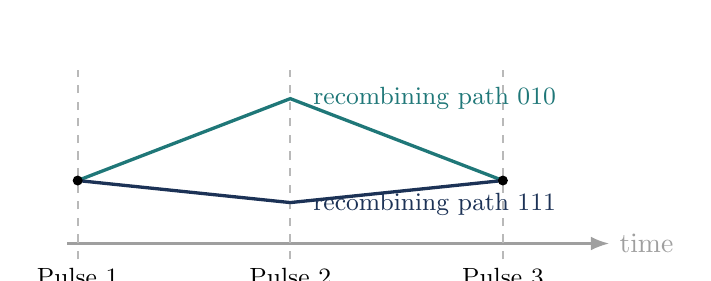
\begin{tikzpicture}[>=Latex,x=1.35cm,y=.80cm,thick]
\draw[->,gray!75] (-.1,0)--(5,0) node[right]{time};
\foreach \x/\lab in {0/{Pulse 1},2/{Pulse 2},4/{Pulse 3}} {
\draw[gray!55,dashed] (\x,-.25)--(\x,2.75);
\node[below,font=\small] at (\x,-.22) {\lab};}
\draw[teal,very thick] (0,1)--(2,2.30)--(4,1);
\draw[navy,very thick] (0,1)--(2,.65)--(4,1);
\node[teal,right,font=\small] at (2.12,2.30) {recombining path 010};
\node[navy,right,font=\small] at (2.12,.63) {recombining path 111};
\fill[black] (0,1) circle (1.8pt);
\fill[black] (4,1) circle (1.8pt);
\end{tikzpicture}
\end{center}
The drawing is schematic, not a quantitative plot of space, time, or momentum.
This path selection assumes adequate spatial separation of unwanted
wave packets and a readout that does not reintroduce their interference.
Additional momentum orders or a different Raman output selection can invalidate
this simplification.

\subsection{Quantum amplitudes, not probabilities, must interfere}

Define
\begin{equation}
 P_{010}=(1-a)b(1-c),\qquad P_{111}=abc.
\end{equation}
Their complex path amplitudes are
\begin{equation}
\mathcal A_{010}=\sqrt{P_{010}}e^{i\phi_{010}},\qquad
\mathcal A_{111}=\sqrt{P_{111}}e^{i\phi_{111}}.
\end{equation}
The recombined probability is
\begin{align}
P_{\rm main}
 &=|\mathcal A_{010}+\mathcal A_{111}|^2\\
 &=P_{010}+P_{111}+2\sqrt{P_{010}P_{111}}\cos\varphi,
\end{align}
where $\varphi=\phi_{111}-\phi_{010}$ is the scanned interferometer phase.
Adding the phase-independent unwanted paths, we obtain
\begin{equation}\label{eq:singlefringe}
P_-(\varphi)=P_{010}+P_{111}+P_{100}+P_{001}
+2\sqrt{P_{010}P_{111}}\cos\varphi.
\end{equation}
Comparing with $P_-=B_{\rm atom}+A_{\rm atom}\cos\varphi$ gives
\begin{align}
 B_{\rm atom}&=P_{010}+P_{111}+P_{100}+P_{001},\label{eq:bsum}\\
 A_{\rm atom}&=2\sqrt{P_{010}P_{111}}.\label{eq:asum}
\end{align}
Thus $B$ is the sum of \emph{phase-independent} populations, whereas $A$ is
an interference contribution.

\subsection{Algebraic derivation of $B_{\rm atom}$, step by step}

Substitute the four path probabilities:
\begin{align}
B_{\rm atom}={}&(1-a)b(1-c)+abc\\
&+a(1-b)(1-c)+(1-a)(1-b)c.
\end{align}
Expand each term separately:
\begin{align*}
(1-a)b(1-c)&=b-ab-bc+abc,\\
abc&=abc,\\
a(1-b)(1-c)&=a-ab-ac+abc,\\
(1-a)(1-b)c&=c-ac-bc+abc.
\end{align*}
Collect like terms:
\begin{equation}
 B_{\rm atom}=a+b+c-2ab-2ac-2bc+4abc.
\end{equation}
Factor the expression:
\begin{align}
 B_{\rm atom}
 &=b+(a+c-2ac)-2b(a+c-2ac)\\
 &=b+(a+c-2ac)(1-2b).
\end{align}
\begin{keybox}
\begin{equation}\label{eq:bfinal}
\boxed{B_{\rm atom}=b+(a+c-2ac)(1-2b).}
\end{equation}
\end{keybox}
This equation is \emph{derived} from the selected two-state closed-path
model and the output-port definition; it is not an empirical fit.

\subsection{Derivation of the fringe amplitude}

Similarly,
\begin{align}
A_{\rm atom}
 &=2\sqrt{(1-a)b(1-c)\cdot abc}\\
 &=2b\sqrt{a(1-a)c(1-c)}.
\end{align}
\begin{keybox}
\begin{equation}\label{eq:afinal}
\boxed{A_{\rm atom}=2b\sqrt{a(1-a)c(1-c)}.}
\end{equation}
\end{keybox}
For ideal values $a=c=1/2$, $b=1$, we recover $B_{\rm atom}=1/2$
and $A_{\rm atom}=1/2$, hence $P_-(\varphi)=(1+\cos\varphi)/2$.
The sign of the interference term depends on the phase convention; the
absolute amplitude and baseline do not.

\section{What is $f_{\Tat}$? The atomic distribution from first principles}

\subsection{Thermal velocity distribution in one dimension}

Assume a nondegenerate, approximately thermal cloud. With zero mean velocity,
a transverse velocity component obeys the Maxwell--Boltzmann Gaussian
probability density
\begin{equation}\label{eq:fv1d}
\boxed{f_{\Tat}(v_x)=\sqrt{\frac{m}{2\pi\kb\Tat}}
\exp\left(-\frac{m v_x^2}{2\kb\Tat}\right).}
\end{equation}
Compare this with a normalized one-dimensional Gaussian
\begin{equation}
 f(v_x)=\frac{1}{\sqrt{2\pi}\sigma_v}
 \exp\left(-\frac{v_x^2}{2\sigma_v^2}\right).
\end{equation}
It follows that
\begin{equation}\label{eq:sv}
\boxed{\sigma_v=\sqrt{\frac{\kb\Tat}{m}}.}
\end{equation}
A higher temperature means a broader velocity distribution. For a nonzero
mean velocity, replace $v_x^2$ with $(v_x-\bar v_x)^2$.

\subsection{Two transverse dimensions}

Assume the two transverse velocity components are independent and have equal
temperature. Multiplying their Gaussian probability densities gives
\begin{equation}\label{eq:fv2d}
\boxed{f_{\Tat}(v_x,v_y)=\frac{m}{2\pi\kb\Tat}
\exp\left[-\frac{m(v_x^2+v_y^2)}{2\kb\Tat}\right].}
\end{equation}
The previously reported axial velocity spread (equivalent to approximately
\SI{90}{nK}) describes \emph{another} distribution. It must not be substituted
for the measured transverse temperature.

\subsection{Initial cloud position distribution}

Assume a centered, isotropic Gaussian initial transverse position with
one-axis RMS width $\sigma_0$:
\begin{equation}\label{eq:fr0}
 f_0(x_0,y_0)=\frac{1}{2\pi\sigma_0^2}
 \exp\left[-\frac{x_0^2+y_0^2}{2\sigma_0^2}\right].
\end{equation}
If initial positions and velocities are independent, the joint phase-space
probability density is the product
\begin{keybox}
\begin{equation}\label{eq:f4d}
\boxed{\begin{aligned}
f_{\Tat}(x_0,y_0,v_x,v_y)
={}&\frac{1}{2\pi\sigma_0^2}
 \exp\left[-\frac{x_0^2+y_0^2}{2\sigma_0^2}\right]\\
&\times\frac{m}{2\pi\kb\Tat}
 \exp\left[-\frac{m(v_x^2+v_y^2)}{2\kb\Tat}\right].
\end{aligned}}
\end{equation}
\end{keybox}
This distribution is normalized over all four coordinates:
\begin{equation}
\int_{\mathbb R^2}\dd^2\bm r_0\int_{\mathbb R^2}\dd^2\bm v_\perp\;
 f_{\Tat}(\bm r_0,\bm v_\perp)=1.
\end{equation}
The assumption of zero initial position--velocity correlation is a modelling
assumption; it may not hold for every launch or state-selection sequence.

\subsection{Ballistic expansion of a Gaussian cloud}

Without significant transverse acceleration,
\begin{equation}
 x(t)=x_0+v_x t,\qquad y(t)=y_0+v_y t.
\end{equation}
For independent zero-mean Gaussians, variances add:
\begin{equation}\label{eq:cloudsigma}
\boxed{\sigma_r^2(t)=\sigma_0^2+\frac{\kb\Tat}{m}t^2.}
\end{equation}
The corresponding \emph{position-only} probability density at time $t$ is
\begin{equation}\label{eq:frt}
\boxed{f_{\Tat}(x,y;t)=\frac{1}{2\pi\sigma_r^2(t)}
\exp\left[-\frac{x^2+y^2}{2\sigma_r^2(t)}\right].}
\end{equation}
Use the four-dimensional joint density when following the \emph{same atom}
through all three pulses. The reduced two-dimensional density is sufficient
for a spatial average at a single instant.

\subsection{Conditional cloud dimensions for MIGA21 and MIGA22}

With negligible initial cloud size and $t_c\simeq\SI{0.4305}{s}$,
\begin{equation}
\sigma_r(t_c)\simeq t_c\sqrt{\kb\Tat/m}.
\end{equation}
Using the temperatures in Table~1 gives approximately
\begin{center}
\begin{tabular}{lcc}\toprule
Quantity & MIGA22 & MIGA21\\\midrule
Transverse velocity RMS & \SI{15.77}{mm/s} & \SI{13.37}{mm/s}\\
Cloud one-axis RMS at $t_c$ & \SI{6.79}{mm} & \SI{5.76}{mm}\\\bottomrule
\end{tabular}
\end{center}
These are predictions of the free-expansion Gaussian assumption, not directly
measured sizes at the Bragg pulses.

\section{Gaussian Bragg coupling and ensemble-averaged $B(\Tat)$}

\subsection{Position-dependent two-photon Rabi frequency}

For an ideal centered and well-overlapped Gaussian Bragg beam,
\begin{equation}\label{eq:gaussianI}
I(r)=I_0\exp(-2r^2/w^2),\qquad r^2=x^2+y^2.
\end{equation}
In the simplified far-detuned, two-photon picture, take the effective
coupling to be proportional to this intensity:
\begin{equation}\label{eq:gaussianOmega}
\Omega(r)=\Omega_0\exp(-2r^2/w^2).
\end{equation}
If the transverse motion during a short pulse can be neglected,
\begin{equation}
\theta_j(r)=\theta_{j,0}\exp(-2r^2/w^2).
\end{equation}
The local transition probabilities are therefore
\begin{align}
a(r)&=\sin^2\left[\frac{\theta_{1,0}}2 e^{-2r^2/w^2}\right],\\
b(r)&=\sin^2\left[\frac{\theta_{2,0}}2 e^{-2r^2/w^2}\right],\\
c(r)&=\sin^2\left[\frac{\theta_{3,0}}2 e^{-2r^2/w^2}\right].
\end{align}
The center pulse areas $\theta_{j,0}$ are held \emph{fixed} when evaluating
temperature fluctuations. \textbf{Do not recalibrate the $20\%$ and $40\%$
transition efficiencies at each perturbed temperature}: that would partially
remove the response we wish to estimate.

For a realistic Blackman pulse, $\theta_{j,0}$ is the time integral of its
actual effective Rabi envelope. Within the strictly resonant two-state model,
changing the envelope at constant area leaves the transition probability
unchanged; multiport and finite-detuning physics breaks this equivalence.

\subsection{An important Gaussian intensity check}

Spatially averaging the normalized intensity over the expanded Gaussian cloud
gives
\begin{align}
\frac{\av I}{I_0}
&=\int\dd x\dd y\;f_{\Tat}(x,y;t_c)e^{-2(x^2+y^2)/w^2}\\
&=\boxed{\frac{1}{1+4\sigma_r^2(t_c)/w^2}}.
\end{align}
The conditional result is approximately $43.9\%$ for MIGA22 and $52.1\%$
for MIGA21. \emph{Average intensity is not equal to Bragg transition efficiency.}
In particular, because $\sin^2$ is nonlinear,
$\av{\sin^2(\theta/2)}$ is generally not
$\sin^2(\av\theta/2)$.

\subsection{Averaging the single-atom baseline over the cloud}

One atom at transverse position $\bm r$ contributes
\begin{equation}
B_{\rm atom}(\bm r)=b(\bm r)+
 [a(\bm r)+c(\bm r)-2a(\bm r)c(\bm r)][1-2b(\bm r)].
\end{equation}
The cloud baseline is its probability-weighted average:
\begin{keybox}
\begin{equation}\label{eq:Bxy}
\boxed{B(\Tat)=\int_{\mathbb R^2} f_{\Tat}(x,y;t_c)
 B_{\rm atom}(x,y)\,\dd x\,\dd y.}
\end{equation}
\end{keybox}
If all atoms have the same scanned phase offset, the cloud fringe amplitude is
similarly $A=\int f_{\Tat} A_{\rm atom}\,\dd x\,\dd y$.
More generally, when atoms carry different diffraction phases
$\delta\phi(x,y)$, the \emph{complex} fringe coefficient must be averaged:
\begin{equation}\label{eq:complexharmonic}
\mathcal C(\Tat)=\int f_{\Tat}(x,y;t_c)A_{\rm atom}(x,y)
 e^{i\delta\phi(x,y)}\dd x\dd y,\quad
A=|\mathcal C|,\quad\Phi=\arg\mathcal C.
\end{equation}
Our simplified baseline calculation does not evaluate this real diffraction
phase $\Phi$.

\subsection{Reducing the centered two-dimensional integral to one dimension}

For a circularly symmetric cloud and beam, introduce polar coordinates
$x=r\cos\alpha$, $y=r\sin\alpha$, with
$\dd x\,\dd y=r\,\dd r\,\dd\alpha$.
Then
\begin{align}
B(\Tat)&=\int_0^{2\pi}\dd\alpha\int_0^\infty
\frac{r}{2\pi\sigma_r^2}
 e^{-r^2/(2\sigma_r^2)}B_{\rm atom}(r)\,\dd r\\
&=\int_0^\infty\frac{r}{\sigma_r^2}
 e^{-r^2/(2\sigma_r^2)}B_{\rm atom}(r)\,\dd r.
\end{align}
Therefore
\begin{keybox}
\begin{equation}\label{eq:Bradial}
\boxed{\begin{aligned}
B(\Tat)=\int_0^\infty &\frac{r}{\sigma_r^2(\Tat)}
 e^{-r^2/[2\sigma_r^2(\Tat)]}\\
&\times\Big\{b(r)+[a(r)+c(r)-2a(r)c(r)][1-2b(r)]\Big\}\,\dd r.
\end{aligned}}
\end{equation}
\end{keybox}
If the first and third splitter pulses have equal local probabilities,
$a(r)=c(r)$, this becomes
\begin{equation}\label{eq:Bradialsym}
\boxed{B(\Tat)=\int_0^\infty \frac{r}{\sigma_r^2}
 e^{-r^2/(2\sigma_r^2)}\left[b(r)+2a(r)(1-a(r))(1-2b(r))\right]\dd r.}
\end{equation}
This is the \emph{fast radial model} used by default in the companion GUI.

\subsection{More accurate: follow each atom at three pulse times}

A single atom moves during the $20$-ms interferometer sequence. Its
transverse coordinates at the three pulse centers are
\begin{equation}
\bm r_j=\bm r_0+\bm v_\perp t_j,
\qquad(t_1,t_2,t_3)=(t_c-\Tai,t_c,t_c+\Tai).
\end{equation}
The local transition probabilities must then be evaluated as
$a=a(\bm r_1)$, $b=b(\bm r_2)$, $c=c(\bm r_3)$. The full Gaussian
phase-space average becomes
\begin{keybox}
\begin{equation}\label{eq:B4d}
\boxed{\begin{aligned}
B(\Tat)=\int_{\mathbb R^2}\dd^2\bm r_0
\int_{\mathbb R^2}\dd^2\bm v_\perp\;
 f_{\Tat}(\bm r_0,\bm v_\perp)
 \Big\{b+[a+c-2ac](1-2b)\Big\}.
\end{aligned}}
\end{equation}
\end{keybox}
If only a subset of the atoms is accepted by the actual readout, insert the
corresponding spatial or velocity acceptance weight $W$ and normalize by its
integral. The optional effective acceptance parameter in the GUI is not a
measurement of that real detection function.

\section{Temperature sensitivity $K_T=\partial B/\partial\Tat$}

\subsection{The simplest method: central finite differences}

Once the model calculates $B(\Tat)$, define
\begin{equation}\label{eq:KT}
\boxed{K_T=\frac{\partial B}{\partial\Tat}.}
\end{equation}
Estimate it with a central difference:
\begin{equation}\label{eq:KTdiff}
\boxed{K_T\simeq\frac{B(\Tat+\Delta\Tat)-B(\Tat-\Delta\Tat)}{2\Delta\Tat}.}
\end{equation}
For example, using $\Delta\Tat=0.01\,\mu\mathrm K$,
\begin{align}
K_{22}&\simeq[B(2.609)-B(2.589)]/0.020,\\
K_{21}&\simeq[B(1.879)-B(1.859)]/0.020,
\end{align}
with all temperatures measured in $\mu$K. Hold the optical powers, center
pulse areas, phase conventions, beam center, and readout acceptance fixed;
\emph{only} the temperature-dependent distribution changes.

\subsection{Analytic derivative in the radial model}

Let
\begin{equation}
 s(\Tat)=\sigma_r^2(\Tat)=\sigma_0^2+\frac{\kb\Tat}{m}t_c^2,
 \qquad g(r;s)=\frac r{s}e^{-r^2/(2s)}.
\end{equation}
For a fixed local pulse response $B_{\rm atom}(r)$,
\begin{align}
\frac{\partial g}{\partial s}
 &=g(r;s)\left(-\frac1s+\frac{r^2}{2s^2}\right),\\
\frac{\dd s}{\dd\Tat}&=\frac{\kb t_c^2}{m}
 \qquad(\Tat\text{ expressed in kelvin}).
\end{align}
Consequently,
\begin{keybox}
\begin{equation}\label{eq:KTanalytic}
\boxed{K_T=\frac{\kb t_c^2}{m}
 \int_0^\infty\frac r{s}e^{-r^2/(2s)}
 \left(-\frac1s+\frac{r^2}{2s^2}\right)
 B_{\rm atom}(r)\,\dd r.}
\end{equation}
\end{keybox}
For a derivative per $\mu$K rather than per kelvin, multiply the right-hand
side by $10^{-6}$.

A credible numerical result should survive three tests: halve the temperature
finite-difference step, increase the quadrature order, and compare the
modelled baseline and amplitude to actual measured fringes. Numerical
convergence is \emph{not} the same as model validity.

\section{From baseline sensitivity to mid-fringe phase Allan deviation}

\subsection{Linearizing the measured fringe}

Write the normalized signal as
\begin{equation}\label{eq:fringe}
P(\phi;\Tat)=B(\Tat)+A(\Tat)\cos[\phi+\Phi(\Tat)].
\end{equation}
At an ideal mid-fringe working point, the argument of the cosine is $\pi/2$.
For small changes, the first-order output variation is
\begin{equation}
 \delta P\simeq\delta B-A\,\delta\Phi.
\end{equation}
If phase is inferred from population using \emph{fixed} reference values
$B_0,A_0$, the apparent readout-phase fluctuation is
\begin{equation}\label{eq:appphase}
\delta\phi_{\rm read}\simeq\delta\Phi-\frac{\delta B}{A_0}.
\end{equation}
The sign depends on the chosen fringe-slope convention. When studying only
baseline noise, with $\delta\Phi=0$,
\begin{keybox}
\begin{equation}\label{eq:appallan}
\boxed{\sigma_{\phi}^{\rm app}\simeq
 \frac{|K_T|\,\sigma_\Tat}{A_{\rm meas}}.}
\end{equation}
\end{keybox}
At the exact mid-fringe point, the term linear in $\delta A$ is multiplied
by $\cos(\pi/2)=0$. Away from mid-fringe, amplitude fluctuations can also
contribute. True diffraction-phase and baseline responses driven by the
same temperature change must be combined with their signs \emph{before}
computing the noise variance.

\subsection{MIGA22: conditional \SI{58.0}{mrad} example}

A previous \emph{assumed spatial-response model}, not an independent
experimental measurement, gave
$K_{22}\simeq-0.0672\,(\mu\mathrm K)^{-1}$. Taking
$\sigma_{\Tat,22}=0.151\,\mu\mathrm K$ gives
\begin{equation}
\sigma_{B,22}=0.0672\times0.151=0.0101472.
\end{equation}
With the measured absolute amplitude $A_{22}=0.175$,
\begin{equation}
\boxed{\sigma_{\phi,22}^{\rm app}=
 \frac{0.0101472}{0.175}=0.057984\,\mathrm{rad}
 \simeq\SI{58.0}{mrad}.}
\end{equation}

\subsection{MIGA21: conditional \SI{46.1}{mrad} example}

A previous assumed model gave
$K_{21}\simeq-0.0889\,(\mu\mathrm K)^{-1}$.
Using $\sigma_{\Tat,21}=0.109\,\mu\mathrm K$,
\begin{equation}
\sigma_{B,21}=0.0889\times0.109=0.0096901.
\end{equation}
With the \emph{updated measured} amplitude $A_{21}=0.210$,
\begin{equation}
\boxed{\sigma_{\phi,21}^{\rm app}=
 \frac{0.0096901}{0.210}=0.046143\,\mathrm{rad}
 \simeq\SI{46.1}{mrad}.}
\end{equation}

\subsection{Differential noise from two independent atom sources}

If temperature fluctuations of MIGA21 and MIGA22 have negligible
cross-covariance at the Allan averaging time under consideration, the
differential Allan variance is the sum of the two variances:
\begin{equation}
\sigma_{\Delta\phi,\Tat}^2
=\sigma_{\phi,22}^2+\sigma_{\phi,21}^2.
\end{equation}
Thus
\begin{keybox}
\begin{equation}\label{eq:diffans}
\boxed{\sigma_{\Delta\phi,\Tat}^{\rm app}
\simeq\sqrt{58.0^2+46.1^2}\,\mathrm{mrad}
\simeq\SI{74.1}{mrad}.}
\end{equation}
\end{keybox}
These estimates are linear propagation of previously assumed $K_T$ values.
The single-cloud temperature width, temperature Allan deviation, and
shot-to-shot baseline Allan deviation are \emph{different quantities}; one
must not interchange them. If temperature fluctuations are correlated between
sources, include the covariance term rather than adding in quadrature.

\section{Physical limitations and MIGA21 over-rotation}

\subsection{Over-rotation is not automatically a negative slope}

For a single atom,
\begin{equation}
\frac{\partial p}{\partial\theta}=\frac12\sin\theta.
\end{equation}
When $\pi/2<\theta<\pi$, the pulse is over a nominal $\pi/2$ area but
the transfer probability is still increasing. Only above $\pi$ does it start
decreasing. Because $B(\Tat)$ involves both the three transition
probabilities and their temperature-dependent statistical weights, the sign of
$K_T$ cannot be inferred from one local $\partial p/\partial\theta$.
The companion GUI therefore allows different splitter and mirror Rabi branches.

\subsection{A strict consistency bound of the ideal closed-path model}

From Eq.~\eqref{eq:afinal}, and since $a(1-a)\leq1/4$ and
$c(1-c)\leq1/4$,
\begin{equation}
 A_{\rm atom}\leq b/2.
\end{equation}
Averaging over the \emph{same normalized sample} gives
\begin{equation}\label{eq:bound}
\boxed{A\leq\av b/2.}
\end{equation}
Thus if the MIGA21 mean mirror efficiency were precisely $0.40$ for the
\emph{same} atom sample and readout normalization, this model would require
$A\leq0.20$, whereas the measured amplitude is $0.210$.
This does \emph{not} invalidate the measurement: it shows that the joint
assumptions of the simplified model, efficiency definition, and selected
readout ensemble cannot all hold exactly. In particular, the actual MIGA21
mirror efficiency, spatial/velocity acceptance, Raman readout and normalized
population definition may differ from this idealized construction.

\subsection{Why matching averaged efficiencies does not determine $K_T$}

Knowing $\av a$, $\av b$, $B$, and $A$ does not uniquely recover the full
spatial-velocity distribution, pulse-area distribution, or selection weights.
Multiple physical models can reproduce the same observables and produce
different $\partial B/\partial\Tat$. A mismatch between predicted and
measured $B,A$ is a warning that the calculated noise is conditional. This is
why the companion GUI reports both model predictions and measured fringe
parameters side by side.

\section{Reproducible calculation and GUI connection}

\subsection{One-dimensional Gaussian integral in a convenient variable}

For the radial model, introduce
\begin{equation}
 u=\frac{r^2}{2\sigma_r^2},\qquad
 \frac r{\sigma_r^2}\dd r=\dd u.
\end{equation}
Then
\begin{equation}\label{eq:laguerre}
B(\Tat)=\int_0^\infty e^{-u}
 B_{\rm atom}\!\left(r=\sqrt{2\sigma_r^2u}\right)\,\dd u.
\end{equation}
A Gauss--Laguerre rule evaluates this efficiently as
$B\simeq\sum_j w_j B_{\rm atom}(\sqrt{2\sigma_r^2u_j})$.
The local coupling multiplier becomes
\begin{equation}
 e^{-2r^2/w^2}=e^{-4\sigma_r^2u/w^2}.
\end{equation}
The script \texttt{radial\_demo.py} distributed in the ZIP implements this
calculation directly and can be run with NumPy. A short excerpt is
\begin{lstlisting}[style=mypython]
from numpy.polynomial.laguerre import laggauss
import numpy as np
u, weights = laggauss(80)
sigma2 = sigma0**2 + kB*(temp_uK*1e-6)/mass*flight**2
g = np.exp(-4*sigma2*u/waist**2)
a = np.sin(0.5*theta_split*g)**2
b = np.sin(0.5*theta_mirror*g)**2
c = a # symmetric splitters in this approximation
B_atom = b + (a+c-2*a*c)*(1-2*b)
A_atom = 2*b*np.sqrt(a*(1-a)*c*(1-c))
B = np.dot(weights, B_atom)
A = np.dot(weights, A_atom)
\end{lstlisting}
The pulse areas here are illustrative unless calibrated at the baseline
temperature to the measured \emph{ensemble} efficiencies. The calibrated GUI
script supplied separately does exactly that \emph{once}, and then keeps the
pulse areas fixed while scanning temperature.

\subsection{Calibrating both sources at their nominal temperatures}

Let $\theta_{s,0}$ and $\theta_{m,0}$ denote the on-axis splitter and mirror
pulse areas. At the baseline temperature $\Tat_0$, solve
\begin{equation}\label{eq:calibrate}
\begin{aligned}
\int f_{\Tat_0}(\bm r)\sin^2\left(
\frac{\theta_{s,0}e^{-2r^2/w^2}}{2}\right)\dd^2\bm r
 &=p_{\rm split}^{\rm measured},\\
\int f_{\Tat_0}(\bm r)\sin^2\left(
\frac{\theta_{m,0}e^{-2r^2/w^2}}{2}\right)\dd^2\bm r
 &=p_{\rm mirror}^{\rm measured}.
\end{aligned}
\end{equation}
The nonmonotonic $\sin^2$ dependence can yield several solutions. A
meaningful branch must be chosen using knowledge of the Rabi oscillation
(for example, a peak splitter area just above $\pi/2$ for MIGA21).
The code reports the chosen peak areas in units of $\pi$ and warns if the
selected efficiency is unreachable on the requested branch.

\subsection{Updated GUI default scenario (same simplified radial assumptions)}

A new deterministic radial implementation, with a small
$\sigma_0=\SI{0.25}{mm}$ initial position RMS and the above calibration,
gives representative results approximately as follows. Unlike the historical
rounded $K_T$ values in Section 7, these are calculated within one explicitly
specified numerical model, \emph{not} newly measured data.
\begin{table}[ht]
\centering
\caption{Conditional GUI default scenario; $\theta_s,\theta_m$ independently fitted per source.}
\begin{tabular}{lcc}\toprule
Quantity & MIGA22 & MIGA21\\\midrule
Peak splitter area $\theta_s/\pi$ & $0.583$ & $0.513$\\
Peak mirror area $\theta_m/\pi$ & $0.939$ & $0.796$\\
Predicted $B$ & $0.32038$ & $0.35099$\\
Predicted $A$ & $0.16244$ & $0.15872$\\
Calculated $K_B$ ($\mu\mathrm K^{-1}$) & $-0.06713$ & $-0.08843$\\
Baseline apparent Allan (mrad) & $57.92$ & $45.90$\\\bottomrule
\end{tabular}
\end{table}
The corresponding independent-source differential estimate is
$\sqrt{57.92^2+45.90^2}\simeq\SI{73.90}{mrad}$. The mismatch with measured
$B_{22}=0.2905$, $B_{21}=0.4165$, and measured amplitudes remains significant.
\textbf{These precise numbers demonstrate numerical reproducibility within the
chosen assumptions, not validated experimental accuracy.}

\section{Next model: finite-detuning Blackman pulses and quasi-Bragg multiports}

\subsection{What changes at the two-state level?}

For strictly resonant two-state evolution, only the pulse area
$\theta=\int\Omega(t)\dd t$ matters. Hence replacing a square pulse by a
Blackman envelope of the same effective area does \emph{not} change the
predicted transfer probability or the radial-model $B(\Tat)$.
If a finite velocity-dependent detuning is retained, however, the
Hamiltonian becomes
\begin{equation}
H(t)=\frac\hbar2\begin{pmatrix}
\delta(v_\parallel)&\Omega(t)\\
\Omega(t)&-\delta(v_\parallel)
\end{pmatrix}.
\end{equation}
The Hamiltonians at different times no longer generally commute, so pulse
shape and duration do matter. This is a useful intermediate improvement before
full quasi-Bragg multiport propagation.

\subsection{Blackman envelope and duration convention}

A conventional continuous Blackman window supported on $0\leq t\leq\tau$ is
\begin{equation}\label{eq:blackman}
 s(t)=0.42-0.50\cos\left(\frac{2\pi t}{\tau}\right)
 +0.08\cos\left(\frac{4\pi t}{\tau}\right),
\end{equation}
with $s(t)=0$ outside the window. Its time integral is
$\int_0^\tau s(t)\dd t=0.42\tau$. The distinction between the optical
power FWHM, the Rabi-envelope FWHM, and the numerical support $\tau$ must
be stated explicitly when interpreting measured $30$--$60$--$30\,\mu$s pulses.

\subsection{Multi-momentum-state Hamiltonian}

A basis resolving additional momentum orders can be taken as
\begin{equation}
\ket n=\ket{(2n+1)\hbar k+m v_\parallel},\qquad n=-N,\ldots,N.
\end{equation}
A generic optical-lattice coupling model is
\begin{equation}\label{eq:multiH}
\frac{H(t)}\hbar=
\sum_n\omega_n(v_\parallel)\ket n\bra n
+\frac{\Omega_{\rm lat}(t)}2
\sum_n\left[e^{i\phi_L(t)}\ket{n+1}\bra n+\mathrm{h.c.}\right],
\end{equation}
where the kinetic term is based on
\begin{equation}
\omega_n(v_\parallel)=
\frac{[(2n+1)\hbar k+m v_\parallel]^2}{2m\hbar}
\end{equation}
(up to a common energy reference), and the phase $\phi_L(t)$ incorporates
the laser-frequency convention and any detuning or chirp. More accurate
modelling must retain the actual Blackman temporal envelope, Gaussian spatial
coupling, velocity distribution, output-state selection, and wave-packet
overlap. One must verify convergence in momentum-order cutoff and integration
time step.

\subsection{Quantities needed for a complete gradient-noise estimate}

For each source, one should eventually extract
\begin{equation}
\boxed{\frac{\partial B_i}{\partial\Tat_i},\qquad
\frac{\partial A_i}{\partial\Tat_i},\qquad
\frac{\partial\Phi_i^{\rm true}}{\partial\Tat_i},\qquad
\sigma_{\Delta\phi,\Tat}.}
\end{equation}
At the nominal mid-fringe point, a signed combined readout response is
\begin{equation}
K_{{\rm read},i}=
\frac{\partial\Phi_i^{\rm true}}{\partial\Tat_i}
-\frac{1}{A_i}\frac{\partial B_i}{\partial\Tat_i}.
\end{equation}
The true diffraction-phase and baseline sensitivities are \emph{correlated
responses to the same temperature fluctuation} and must be added with signs,
not combined as independent noise powers. Only after obtaining one signed
$K_{{\rm read},i}$ for each source should the contributions from independent
source temperature fluctuations be combined in quadrature.

\begin{keybox}
\textbf{Conclusion.} The simplified two-state calculation gives a transparent,
reproducible conditional estimate for baseline-to-phase conversion. It does
not determine an experimentally validated $K_T$ from temperature and pulse
efficiencies alone. The GUI is designed to explore this uncertainty while
keeping its assumptions visible; a genuine diffraction-phase budget requires
additional physics and calibration data.
\end{keybox}
\end{document}
